\chapter{Simulation and used memory architectures}

In this chapter I will describe the simulation, environment and agent's reasoning and communication how it is used in later experiments. 

\section{Simulation}

The \emph{simulation} consists of a set of agents, a set of generators and a set of pieces of food. According to given settings it subsequently processes a number of steps, each of which invokes agents' life step and eventually generating new food.

The simulation can also contain a couple of monitors which observe the environment or agents.

\section{Environment}

The environment is a two-dimensional space which contains agents and food. Agents can move around and eat the food which is randomly distributed using the food generators. 

\section{Agent}                                                      
As mentioned previously, an agent is an entity in the environment which moves and interact with the world around. The interaction is done through eating food which is a part of the environment and through communication with other agents. The latter one actually changes agents' beliefs about the environment.

Each agent has his needs which influence his decisions as fulfilling his needs keeps him alive. When his internal variables of needs is higher than \textbf{.....?}

There are four types of agents each of which is different in the way they decide about next step. If one is hungry and sees food (i.e. there is a piece of food in the sight distance) then they choose to go after this food. If there is no desired food around they go searching for it and that is when the agents' actions differ.

\begin{itemize}
\item \emph{random agent} moves randomly around the environment,
\item \emph{pure reactive agent} sees the whole environment, i.e. they always sees a desired piece of food, 
\item \emph{grid agent} implements a memory based on clustering the space into a grid,
\item \emph{GNG agent} implements a memory based on growing neural gas.
\end{itemize}

\section{Communication}

Apart from what agent sees, there is another way how the agents gather information about the environment. They communicate. It is a quite simple way of sharing information. When suggesting an implementation for communication, I had to create a unified protocol which could have been used throughout all types of agents. I tried to keep this communication protocol as simple as possible.

Moreover, although all agents have a knowledge of a sort about the environment, they are not able to answer easily when asked about a specific food location. Since the food appears in environment according to given normal distribution, it is not clear what should be an answer to such question. Several possible kinds of answers follow. 

First and the simplest answer might be the exact X,Y coordinates of the food location as it is stored in agent's mind. Additionally, there would be a noise added to such answer, keeping in mind that the answer should not be perfect and there is always a distortion and imperfection in our answers based on how a person is certain about his answer.
                                              
Another way, and perhaps a more plausible one, might be answering with a direction (an angle) with an approximate distance. What both the X, Y answer and the latter information have in common is that the answers are hard to combine with the learning method used in GNG memory. GNG works with samples of data which subsequently influence the neural network. Both kinds of answers could be used if agents would ask more often or the agent's answer would be a sample of points straight away.

So I have implemented a communication model (see \ref{solution:decision}) whereby an answer consists of a small set of points. Each point is generated according to agent's knowledge. When an agent is asked, first he uses his either GNG memory, or grid memory to estimate the Gaussian distribution of the food resource and then randomly generates the points using the estimated distribution.

\begin{figure}
  \centering                                
  \includegraphics[scale=0.7]{diagrams/solution/communication.eps}    
  \caption{Simple communication protocol}
  \label{solution:communication}
\end{figure}

\section{Decision making}

While searching for food, each type of the agent makes the decision where to go next. This process is either done randomly or following one's knowledge of the environment. A simple diagram of decision making follows.

\begin{figure}
  \centering                                
  \includegraphics[scale=0.7]{diagrams/solution/decision-flowchart.eps}    
  \caption{How the agent decides what to do next}
  \label{solution:decision}
\end{figure}

The diagram \ref{solution:decision} shows how an agents decides what to do. In fact it is common for all types of agents described in this thesis, although the first step "Put known food location into memory" is omitted in case of \emph{random} and \emph{PR agents}. 

First an agent puts into his memory known food locations. These are locations which he either sees, or remembers from the last simulation step. After that he checks his internal variables to see whether he is hungry or not. If he is hungry, he tries to decide where his desired food resource is. He uses his memory, sight and eventually communication with other agents. 

The output of this process is a group of possible locations from which he chooses the closest one and head towards it. If he occures at the position where the desired food also is, he eats it. Throught the decision flow there are two moments, when the agent does not know what to do and then he moves randomly: when he does not need to eat anything and when he cannot find the the path to the food resource.

\section{Memories}

There are two types of memory which should allow agents to improve their lifespan compared to a random agent. Those are memories based on a growing neural gas and a spatial grid.     

The \emph{GNG memory} uses a self-teaching neural network which has been described in \ref{usedalgo:gng}. The neural network allows the agent to learn the approximate location where the food is distributed. Each kind of food is given a single neural network which tries to learn the distribution reflecting the data inputs..

The \emph{grid memory} divides the environment into a grid in order to simplify the space and to restrict the total size of the data structure used to describe the space.




